\section{Introduzione}
L'applicazione sviluppata vuole offrire un meccanismo per monitorare l'ambiente e il dispositivo a difesa da intrusioni indesiderate.
 \textit{SecureIt} è stata pensata come un'applicazione in grado di trasformare un dispositivo Android in un sistema d'allarme da posizionare opportunisticamente all'interno della propria abitazione in grado di avvisare l'utente di possibili intrusioni, fornirgli dati relativi all'intrusione ed in grado di fornire informazioni riguardanti la locazione del dispositivo stesso.\\

A differenza di altre applicazioni già presenti nel mercato che focalizzano il loro meccanismo di controllo ambientale per garantire un solo tipo di sicurezza, \textit{SecureIt} tenta di sfruttare al massimo le potenzialità di un dispositivo per offrire meccanismi di protezione ad ampio spettro:
\begin{itemize}
  \item Utilizza l'accelerometro per determinare movimenti del dispositivo. Questo meccanismo è in grado di rilevare qualora qualche intruso urti o prenda volontariamente il dispositivo
  \item Utilizza la fotocamera per rilevare e registrare movimento all'interno dell'ambiente in cui è posizionato il dispositivo. Qualora un intruso passi davanti alla fotocamera del dispositivo, tale movimento verrà rilevato
  \item Utilizza il microfono per rilevare e registrare rumori sospetti. Questo meccanismo è in grado di rilevare intrusi qualora non siano abbastanza cauti da non causare rumori
  \item Utilizza SMS per avvisare l'utente di aver rilevato una possibile intrusione
  \item Utilizza opportunisticamente reti WiFi e 3G per memorizzare su un server apposito le informazioni registrate (immagini o audio) relative all'intrusione
  \item Utilizza opportunisticamente servizi di localizzazione e collegamenti bluetooth con altri dispositivi per determinare la posizione del dispositivo. Qualora un intruso prelevi il dispositivo, il dispositivo stesso segnalerà ad intervalli regolari la propria posizione al server predisposto a raccogliere tali informazioni o i dispositivi scoperti tramite bluetooth si faranno portavoce per segnalare la posizione in cui è stato incontrato il dispositivo
\end{itemize}

Ovviamente l'utilizzo simultaneo di tutti questi meccanismi può essere oneroso per il dispositivo o addirittura impossibile qualora il dispositivo difetti di alcune componenti (fotocamera rotta, assenza di rete, etc.).\\
All'avvio dell'applicazione viene quindi richiesto all'utente di selezionare i meccanismi che intende attivare. 
\begin{figure}[!ht]
\begin{center}
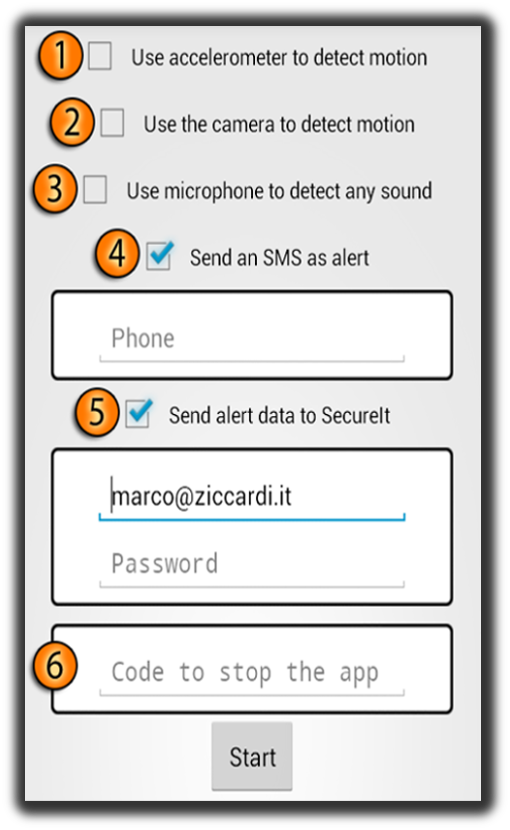
\includegraphics[scale=.3]{./../wireless/resources/config.png}
\caption{Schermata iniziale per la configurazione dell'applicazione.}
\label{fig:SchermataIniziale}
\end{center}
\end{figure}

\noindent Figura \ref{fig:SchermataIniziale} illustra tale schermata e le varie opzioni che è possibile selezionare:
\begin{enumerate}
  \item Abilitare l'utilizzo dell'accelerometro. Qualora non fosse disponibile l'accelerometro questa opzione non sarebbe visualizzata
  \item Abilitare l'utilizzo della fotocamera. Qualora si decida di utilizzare la fotocamera è possibile:
  \begin{itemize}
    \item Scegliere quale fotocamera utilizzare qualora siano disponibili più fotocamere
    \item Scegliere se abilitare il flash
    \item Scegliere la sensibilità con la quale l'applicazione determina il movimento
  \end{itemize}
  \item Abilitare l'utilizzo del microfono. Qualora si decida di utilizzare questa opzione è possibile specificare la sensibilità dell'applicazione verso il rilevamento del rumore
  \item Abilitare l'invio di messaggi SMS al numero specificato qualora venga determinata un'intrusione
  \item Abilitare l'invio delle informazioni raccolte al server incaricato qualora venga determinata un'intrusione. \`E necessario specificare le credenziali con le quali si è noti al server (è necessario essersi precedentemente registrati al server)
  \item Specificare un codice di sblocco per terminare l'applicazione. Solo la persona che ha avviato l'applicazione è in grado di farla terminare correttamente
\end{enumerate}
